% !TeX encoding = UTF-8
\section{Fundamentals}
\subsection{Basic definitions in the graph theory}
Before we start with the proofs of algorithm, let's give some useful definitions in the graph theory:
\begin{definition}
A \textit{graph} is a pair $G = (V, E)$, where $V$ is a set whose elements are called vertices, and $E$ is a set of paired vertices, whose elements are called edges. \cite{graph}
\end{definition}

\begin{definition}
A \textit{$cycle$ $C$} in a graph is a non-empty trail in which the only repeated vertices are the first and last vertices. \cite{Cycle}
\begin{figure}[H] %H为当前位置,!htb为忽略美学标准,htbp为浮动图形
\centering %图片居中
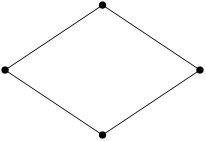
\includegraphics[width=0.2\textwidth]{figure/cycle.png} 
\caption{Cycle $C$} %最终文档中希望显示的图片标题
\label{figure} %用于文内引用的标签
\end{figure}
\end{definition}

\begin{definition}
\textit{$Faces$} of a planar graph are regions bounded by a set of edges and which contain no other vertex or edge. \cite{Face}
\begin{figure}[H] %H为当前位置,!htb为忽略美学标准,htbp为浮动图形
\centering %图片居中
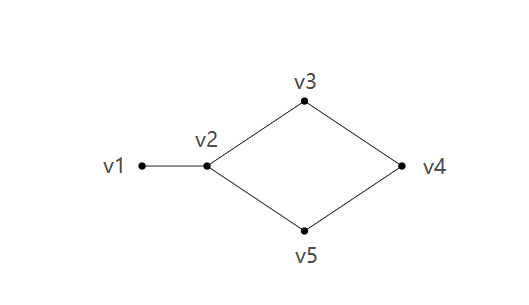
\includegraphics[width=0.2\textwidth]{figure/face.png} 
\caption{Face $F$} %最终文档中希望显示的图片标题
\label{figure} %用于文内引用的标签
\end{figure}
\end{definition}

\begin{definition}
A cycle $C$ is a \textit{facial cycle} in $G$ if it bounds a face in a component in $G$, regardless of whether $F$ itself is a face or not. \cite{dvorak2013threecoloring}
\begin{figure}[H] %H为当前位置,!htb为忽略美学标准,htbp为浮动图形
\centering %图片居中
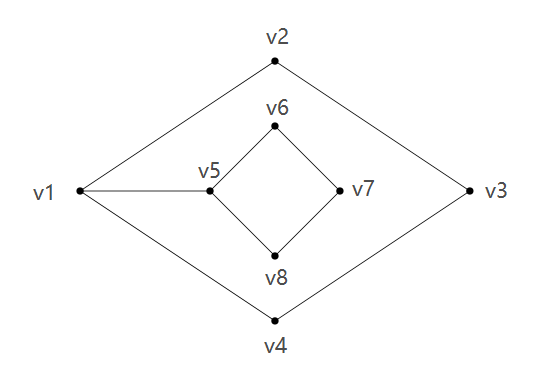
\includegraphics[width=0.2\textwidth]{figure/facialcycle.png} 
\caption{A facial cycle $C$} %最终文档中希望显示的图片标题
\label{figure} %用于文内引用的标签
\end{figure}
\end{definition}

\begin{observation}
A cycle is either a face or a separating cycle.
\end{observation}

\begin{definition}
A cycle $C$ in a connected graph $G$ is a \textit{separating cycle} if the deletion of $C$ from $G$ results in a disconnected graph. \cite{THOMASSEN197857}
\begin{figure}[H] %H为当前位置,!htb为忽略美学标准,htbp为浮动图形
\centering %图片居中
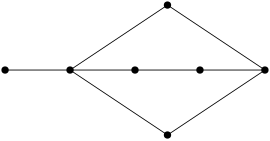
\includegraphics[width=0.2\textwidth]{figure/separating cycle.png} 
\caption{Separating cycle} %最终文档中希望显示的图片标题
\label{figure} %用于文内引用的标签
\end{figure}
\end{definition}

\begin{definition}
Let $G = (V, E)$ be a planar graph: Then a face of $G$ is \textit{incident to an edge} $e$ of $G$ if $e$ is one of those which surrounds the face. Similarly, a face of $G$ is \textit{incident to a vertex} $v$ of $G$ if $v$ is at the end of one of those incident edges. \cite{Incident}
\end{definition}

\begin{definition}
Exactly one region is unbounded, also called \textit{the outer face}, and the others are bounded by cycles in the graph. \cite{Theorem}
\end{definition}

\begin{definition}
An 2-dimensional \textit{open disk of radius $r$} is the collection of points of distance less than $r$ from a fixed point in Euclidean 2-space and an 2-dimensional \textit{closed disk of radius $r$} is the collection of points of distance less equal than $r$ from a fixed point in Euclidean 2-space. \cite{Open_disk}

\begin{figure}[H] %H为当前位置,!htb为忽略美学标准,htbp为浮动图形
\centering %图片居中
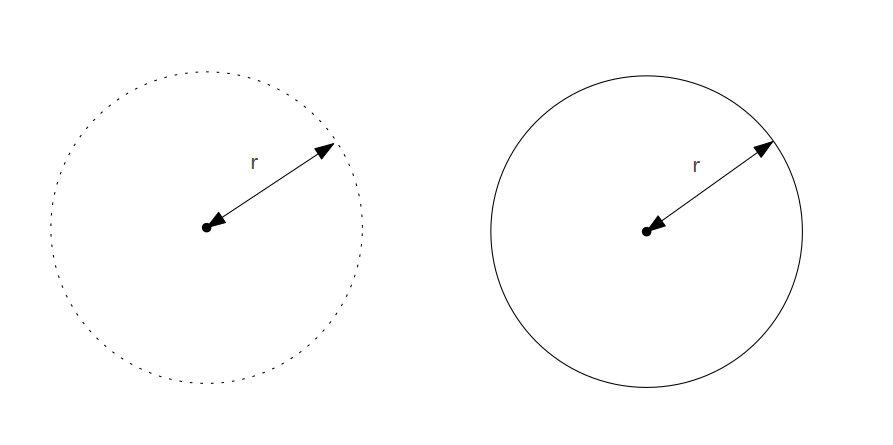
\includegraphics[width=0.7\textwidth]{figure/closeddisk.png} 
\label{figure} %用于文内引用的标签
\caption{Open and close disks of radius $r$}
\end{figure}
\end{definition}

\begin{definition}
An \textit{induced path} in an undirected graph $G$ is a path that is an induced subgraph of $G$. Similarly, \textit{an induced cycle} is a cycle that is an induced subgraph of $G$; induced cycles are also called chordless cycles. \cite{Induced_path}
\end{definition}

\subsection{The core idea}
After knowing these beneficial definitions, we'll bring into totally five reducible configurations, also called \textit{multigrams}. With such multigrams, we can reduce the size of graph $G$ to have a smaller graph $G^{'}$ by identifying some vertices (see definition in the next section). Meanwhile, although we get a smaller graph $G^{'}$, its coloring can be reconstructed to the coloring of $G$ in constant time. The algorithm detects recursively such multigrams with certain constraints so that the size of graph will always get smaller each time until it's so simple to find the corresponding coloring. Next, according to the resulted coloring, we can reconstruct the coloring of its previous graph step by step. In the end, we'll get the proper coloring of the input graph. 

